\documentclass[12pt,a4paper]{article} %hoja A4 y tamño de letra 12pt
\usepackage{setspace}
\onehalfspacing %interlineado 1,5 (no parece el mismo de Word pero es Word el que hace mal eso, este es el posta)
\usepackage[spanish,es-tabla]{babel} %idioma español y "tabla" en lugar de "cuadro"
\usepackage{fontspec}
\setmainfont{Calibri}
%\setmainfont{Times New Roman} %solamente para la primera entrega
%\newfontfamily\myfont{Calibri} %solamente para la primera entrega
\usepackage{datetime}
\usepackage{fancyhdr} %para alinear números de página a la derecha
\usepackage{lipsum}
\renewcommand{\headrulewidth}{0pt}%
\newdateformat{monthyeardate}{
  \monthnamespanish[\THEMONTH]  \THEYEAR}  \makeatletter	
\renewcommand{\monthnamespanish}[1][\month]{%
  \@orgargctr=#1\relax
  \ifcase\@orgargctr
    \PackageError{datetime}{Invalid Month number \the\@orgargctr}{%
      Month numbers should go from 1 to 12}%
    \or Enero%
    \or Febrero%
    \or Marzo%
    \or Abril%
    \or Mayo%
    \or Junio%
    \or Julio%
    \or Agosto%
    \or Septiembre%
    \or Octubre%
    \or Noviembre%
    \or Diciembre%
    \else \PackageError{datetime}{Invalid Month number \the\@orgargctr}{%
      Month numbers should go from 1 to 12}%
  \fi}
\makeatother
\usepackage{amsmath,amsfonts,amssymb}
\usepackage{graphicx} %para figuras
\usepackage[font=footnotesize]{caption} %descripciones de tablas/figuras en 10pt
\graphicspath{ {imagenes/} } %carpeta donde guardar imágenes
\usepackage{luatodonotes}
\setlength{\marginparwidth}{2 cm}
\usepackage[left=3cm,right=2.5cm,top=2.5cm,bottom=2.5cm]{geometry} %márgenes
%\usepackage[sorting=none,maxbibnames=99,isbn=false,doi=false,eprint=false,giveninits=true]{biblatex}
\usepackage[
backend=biber,
sorting=none,
style=numeric-comp
]{biblatex} %referencias
\renewbibmacro{in:}{}
\DeclareNameAlias{default}{last-first}
\addbibresource{referencias.bib} %añade archivo de referencias
\usepackage{tikz}
\usetikzlibrary{calc}
\usetikzlibrary{babel}
\usepackage{titlesec}
\titleformat{\section}{\normalfont\fontsize{16}{19}\bfseries}{\thesection.}{0.5em}{\MakeUppercase} %formato de título
\titleformat{\subsection}{\normalfont\fontsize{14}{16}\bfseries}{\thesubsection.}{0.5em}{\MakeUppercase} %formato de subtítulo
\titleformat{\subsubsection}{\normalfont\fontsize{14}{16}}{\thesubsection.}{0.5em}{} %formato de sub-subtítulo
\let\labelitemi\labelitemii

%Esto se modifica como quieran:
\author{Autor}
\title{Título}
  % mete el contenido del archivo head.tex como preámbulo
%COMILLAS:  “”
\begin{document}
\begin{titlepage}
	%\myfont %solamente para la primera entrega
	\begin{tikzpicture}[remember picture, overlay]
  	\draw[line width = 1pt] ($(current page.north west) + (1cm,-1cm)$) rectangle ($(current page.south east) + (-1cm,2cm)$);
	\end{tikzpicture}
    \begin{center}
	   	   
	   
\includegraphics[width=0.8\textwidth]{logo} 
	          
        \vspace*{1cm}
        \fontsize{18pt}{22pt}\selectfont
        \textbf{INGENIERÍA DE SONIDO}
               
        \vspace{4cm}
        \fontsize{22pt}{26pt}\selectfont
        \textbf{Título\dag}
        
        \vspace{3cm}
        \fontsize{18pt}{22pt}\selectfont
        \textbf{Autor: Nombre Apellido}
        
        \fontsize{16pt}{16pt}\selectfont
        \textbf{Tutor: Nombre Apellido}\par
        \textbf{Co-tutor: Nombre Apellido} %se puede sacar si no hay co-tutor
        
        \vspace{2cm}
        \fontsize{12pt}{14pt}\selectfont
        \textbf{(\dag) Tesis para optar por el título de ingeniero/a de Sonido}
        
        \vspace{1cm}
        
      
        
        \fontsize{14pt}{17pt}\selectfont
        \monthyeardate\today
        
    \end{center}
\end{titlepage} %inserta la portada

% Esta parte setea la numeración (abajo a la izquierda) y la inicia
\pagestyle{fancy}
\fancyhead{}
\fancyfoot{}
\fancyfoot[R]{\thepage}

\tableofcontents % índice
\newpage %comando para salto de página

\begin{flushleft} 
	\fontsize{14pt}{17pt}\selectfont
	\textbf{Resumen}
\end{flushleft}

Acá va el resumen.\par

\begin{footnotesize}
	\textbf{Keywords:} Palabra1, Palabra2, Palabra3, Palabra4, Palabra5.
\end{footnotesize}

\begin{flushleft} 
	\fontsize{14pt}{17pt}\selectfont
	\textbf{Abstract}
\end{flushleft}

Acá va el  abstract.\par

\begin{footnotesize}
	\textbf{Keywords:} Word1, Word2, Word3, Word4, Word5.
\end{footnotesize}


\newpage

%Título (solo para el plan)
%\begin{center}
%	\fontsize{16pt}{17pt}\selectfont
%	\textbf{Título}
%\end{center}

\section{Fundamentación e Introducción.}
Esta es una primera cita en un primer párrafo \cite{Repp2005}.\par
Estas son dos cita en un segundo párrafo \cite{Grootswager2020, Geronazzo2014}.\par
Acá tenemos varias citas en conjunto \cite{Gallant2019, Bridges2020, Anwyl2020, Pronk2020}. \par
Acá hay una cita de una página web usando el campo “author” \cite{Warusfel2002} y acá otra usando el campo “pageowner” \cite{KEMAR}.
Esta es una nota al pie \footnote{Y este es el texto de la nota al pie.}.\par
A continuación puede verse la ecuación \eqref{eq:distancia}:
\begin{equation}\label{eq:distancia}
	d = \sqrt{\sum_{i=1}^{N}{(x_i -y_i})^2 }
\end{equation}

\section{Objetivos}
\subsection{Objetivo general}
Acá va el objetivo principal.\par
\subsection{Objetivo específico}
Lista de objetivos específicos
\begin{itemize}
\item Primer objetivo
\item Segundo objetivo
\item Tercer objetivo, que se divide en:
	\begin{itemize}
		\item Primer sub-objetivo
		\item Segundo sub-objetivo
		\item Tercer sub-objetivo
	\end{itemize}
\item Cuarto objetivo
\end{itemize}

\section{Marco Teórico y Estado del Arte.}
En la Figura \ref{fig:RespFrec} hay un modelo de figura.

\begin{figure}[h]
	\centering
	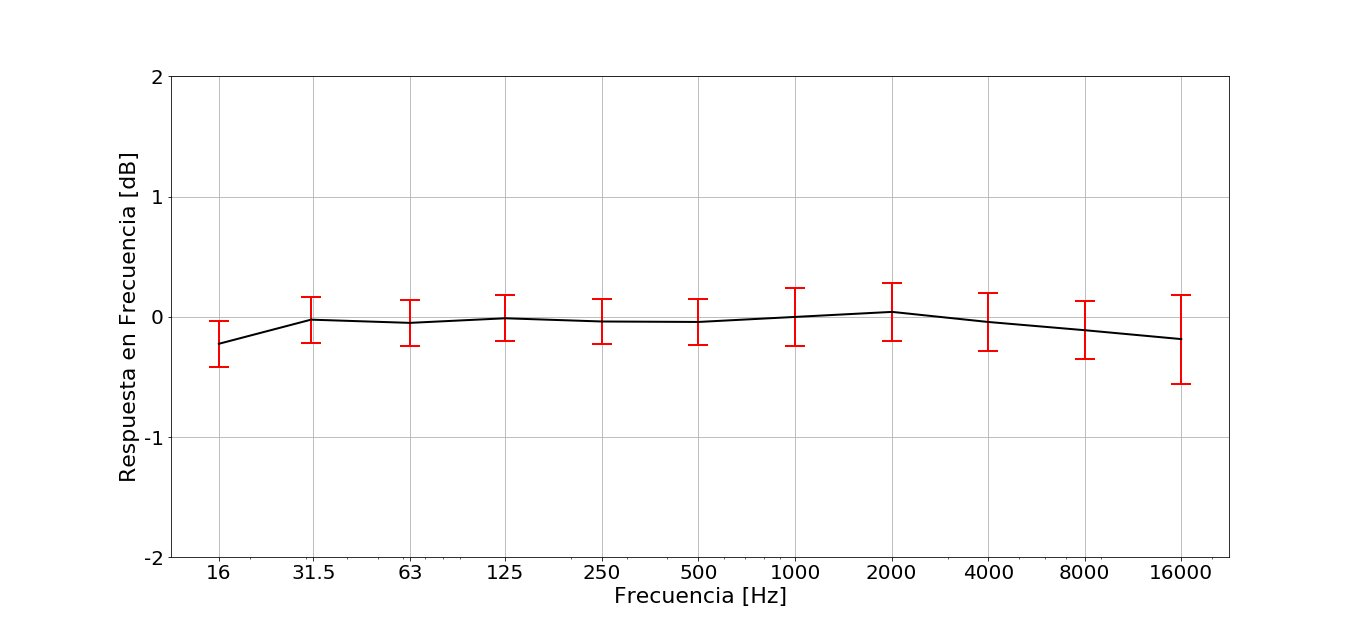
\includegraphics[width=15.5 cm]{RespFrec.jpg}
	\caption[RespFrec]{Figura modelo} 
	\label{fig:RespFrec}
\end{figure}

\section{Diseño de la Investigación.}

\subsection{Diseño prueba objetiva: Definición de Variables.}
En la tabla \ref{tab:HRTFangles} se ve un modelo de tabla.

\begin{table}[h]
	\centering
	\caption{Título de la tabla.}
	\begin{tabular}{ccc}
		\hline
		\textbf{Columna 1}&\textbf{Columna 2}&\textbf{Columna 3}\\\hline
		
		Fila 1 Col 1 & Fila 1 Col 2 & Fila 1 Col 3\\\hline
		Fila 2 Col 1 & Fila 2 Col 2 & Fila 2 Col 3\\\hline
		Fila 3 Col 1 & Fila 3 Col 2 & Fila 3 Col 3\\\hline
	\end{tabular}  
	\label{tab:HRTFangles}
\end{table}

\subsection{Diseño prueba subjetiva: Encuesta y Muestra.}
Acá hay una lista numerada:
\begin{enumerate}
	\item Primero
	\item Segundo:
	\begin{enumerate}
		\item Primero del segundo
		\item Segundo del segundo
		\item Tercero del segundo
	\end{enumerate}
\end{enumerate}

\section{Resultados.}

\section{Discusiones.}

\section{Conclusiones}

\section{Líneas futuras de investigación.}

\section{Cronograma} %solo para plan de tesis
Diagrama de Gantt de modelo.
\begin{figure}[h]
	\centering
	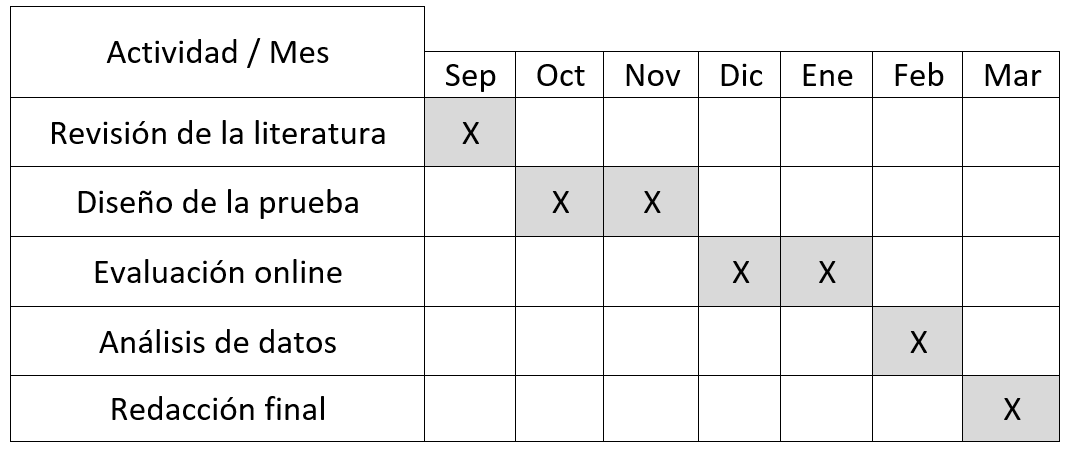
\includegraphics[width=0.8\textwidth]{Cronograma.png}
	\label{fig:Cronograma}
\end{figure}

\newpage
\section{Bibliografía}
\printbibliography[heading=none]

\end{document}